\documentclass[11pt]{article}
\usepackage[left=25mm,right=25mm,top=30mm,bottom=30mm]{geometry}
\usepackage{amsmath} % math
\usepackage{amssymb} % math
\usepackage{graphicx} % to use \includegraphics{}
\usepackage{diagbox} % to make advanced tables
\usepackage{multirow} % to make advanced tables 
\usepackage[hangul]{kotex} % to use Korean
\usepackage{color} % to use color font 
\usepackage[hidelinks]{hyperref} % to insert hyperlinks
\begin{document}
	\begin{center}
		\Large An Introduction to \LaTeX ver 1.9
		
		\normalsize 마지막 작성일 :  \today
		
		공식 웹사이트 : http://gshslatexintro.github.io/gshslatexintro
	\end{center}
\section{기초}
\LaTeX 은 우리가 보통 쓰는 아래아한글이나 Microsoft Word와는 달리, TeXeditor를 통해 문서 코드를 작성하고, 컴파일하여 pdf 문서를 생성해내는 방식으로 문서를 작성하는 방식이다. 코드를 작성하는 방법을 배우는 것이 처음에는 어려울 수 있으나 숙련되고 나면 그 편리함을 이루 말로 다 할 수 없을 정도이다.

\subsection{TeX 편집기}
TeX 편집기(TeXeditor)는 Texmaker, TeXworks, TeXstudio 등등 여러 종류가 있다.\footnote{Eclipse 사용자의 경우 내장된 TeXclipse plugin이 있다고 하지만 여기서는 설명하지 않는다.} TeX 편집기의 목록은 \href{https://en.wikipedia.org/wiki/Comparison_of_TeX_editors}{\textbf{여기}} 에 있으나 입문자에게는 딱히 필요없다. TeXstudio를 사용하기를 추천한다. 

온라인 TeX 편집기도 있다. 특히 \href{https://www.sharelatex.com/}{ShareLaTeX} 와 같은 온라인 TeX 편집기의 경우 Google Docs처럼 tex문서를 동시에 편집할 수 있어서 유용하다.

\begin{figure}
	\begin{center}
		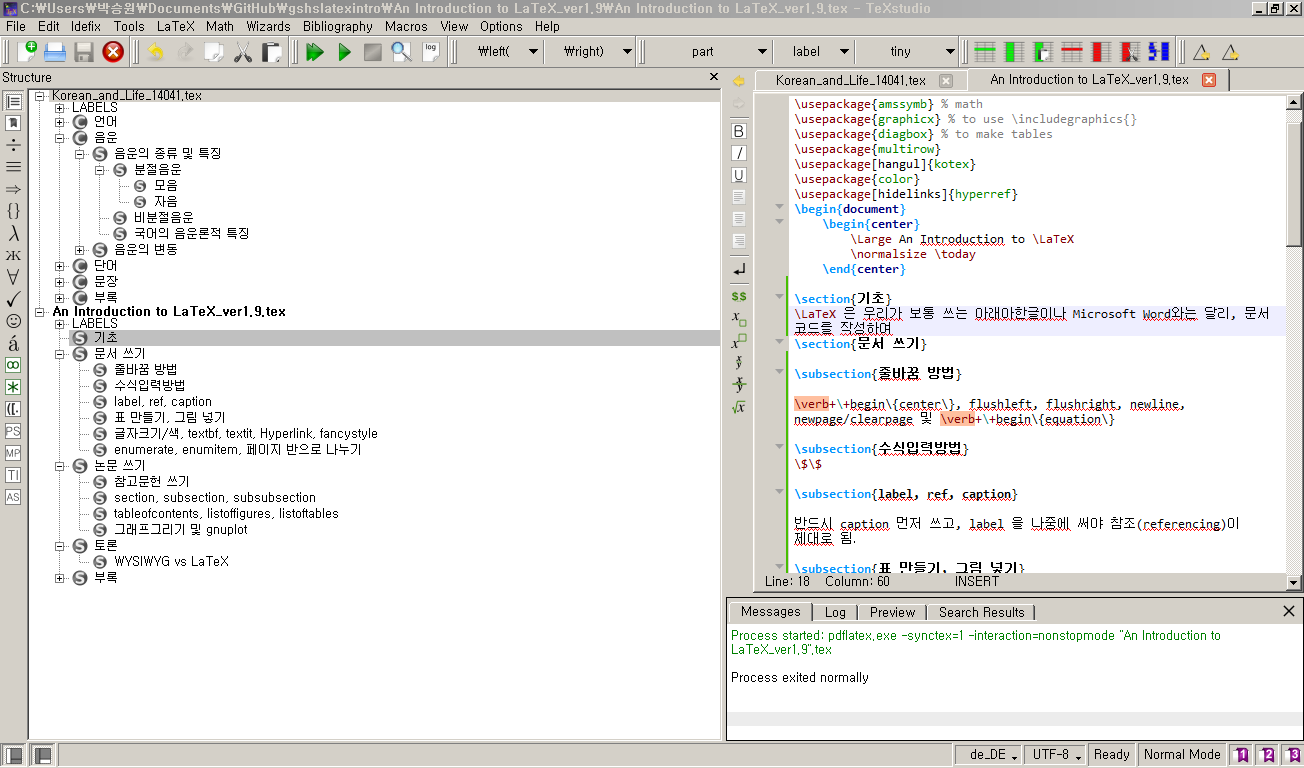
\includegraphics{texstudio.png}
	\end{center}
	\caption{TeXstudio를 이용하여 이 문서를 편집하는 화면}
	\ref{texstudio}
\end{figure}

\section{문서 쓰기}
\LaTeX 문서는 기본적으로 헤더 - 문서 와 같이 구성된다. 이 문서의 헤더는 다음과 같으며, 헤더 다음에는 \verb+\+begin\{document\}와 같이 문서가 시작된다. 모든 모드는 \verb+\+begin\{...\}로 시작하고  \verb+\+end\{...\} 로 끝난다.

\begin{center}
	\verb+\+documentclass[11pt]\{article\}
	
	\verb+\+usepackage[left=25mm,right=25mm,top=30mm,bottom=30mm]\{geometry\}
	
	\verb+\+usepackage\{amsmath\} \% math
	
	\verb+\+usepackage\{amssymb\} \% math
	
	\verb+\+usepackage\{graphicx\} \% to use
	
	\verb+\+includegraphics\{\}
	
	\verb+\+usepackage\{diagbox\} \% to make advanced tables
	
	\verb+\+usepackage\{multirow\} \% to make advanced tables 
	
	\verb+\+usepackage[hangul]\{kotex\} \% to use Korean
	
	\verb+\+usepackage\{color\} \% to use color font 
	
	\verb+\+usepackage[hidelinks]\{hyperref\} \% to insert hyperlinks
\end{center}

\subsection{줄바꿈 방법}

\verb+\+begin\{center\}, flushleft, flushright, newline, newpage/clearpage 및 \verb+\+begin\{equation\}

\subsection{수식입력방법}
\$\$

\subsection{label, ref, caption}

반드시 caption 먼저 쓰고, label 을 나중에 써야 참조(referencing)이 제대로 됨.

\subsection{표 만들기, 그림 넣기}


※첨언 : 인터넷에 \href{www.tablesgenerator.com}{\LaTeX Table Generator} 가 있다. 초반에는 이것을 써도 나쁘지 않을 듯. 

\subsection{글자크기/색, textbf, textit}
\subsection{Hyperlink, fancystyle}

\subsection{enumerate, enumitem, 페이지 반으로 나누기}

\section{논문 쓰기}

\subsection{참고문헌 쓰기}
\begin{center}
\verb+\+begin\{thebibliography\}\{00\}
\verb+\+bibitem\{gshs\}\{http://gs.hs.kr\}

\verb+\+bibitem\{sjgshs\}\{https://student.gs.hs.kr\}
\verb+\+end\{thebibliography\}
\end{center}
\verb+\+cite\{...\} 와 같이 쓰면 참고문헌의 논문 번호가 나온다.

\subsection{section, subsection, subsubsection}
보통 다른 워드프로세서로 논문을 작성할 때 가장 귀찮은 점 중 하나가 절마다 번호를 붙이는 것이다. 하지만 \LaTeX 의 경우 다음의 함수들을 사용하면 된다.

\begin{center}
\verb+\+section\{...\}

\verb+\+subsection\{...\}

\verb+\+subsubsection\{...\}
\end{center}

참고로 subsubsection은 documentclass가 article일 경우 숫자가 나타나지 않고 번호만 나온다. 그림 \ref{section}참조.

\begin{figure}
	\begin{center}
		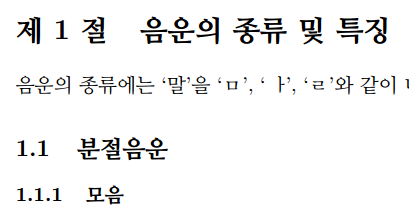
\includegraphics{section_subsection_subsubsection.png}
	\end{center}
	\caption{예시 ㅁㄴㅇㄹ}
	\label{section}
\end{figure}

\subsection{tableofcontents, listoffigures, listoftables}
\LaTeX 은 차례도 자동으로 만들어준다. 다음의 함수들을 사용하면 된다.

\begin{center}
\verb+\+tableofcontents ; 차례(Contents)
	
\verb+\+listoffigures : 그림 차례(List of Figures)
	
\verb+\+lisfoftables : 표 차례(LIst of Tables)
\end{center}


\subsection{그래프그리기 및 gnuplot}

\section{토론}

\subsection{WYSIWYG vs LaTeX}
WYSIWYG(What you see is What you get)

\section{부록}

\subsection{차례}

\tableofcontents
\listoffigures
\listoftables

\subsection{참고 문헌}
\begin{thebibliography}{00}
\bibitem{gshs}{http://gs.hs.kr}
\bibitem{sjgshs}{https://student.gs.hs.kr}
\end{thebibliography}


\end{document}
